\begin{frame}
  \frametitle{Système de communication contrôleur/moniteur}
  \framesubtitle{PCF et objet PCF}
  \begin{itemize}
  \item Protocole de contrôle ferroviaire
    \vspace{1em}
    \begin{itemize}
      \item Format XML
        \vspace{1em}
      \item Balises à identifiant unique
        \vspace{1em}
    \end{itemize}
  \item Objet PCF
    \vspace{1em}
    \begin{itemize}
      \item Éléments décrivants un équipement
        \vspace{1em}
      \item Éléments pour la topographie d'un réseau
        \vspace{1em}
      \item Élément pour l'initialisation
        \vspace{1em}
    \end{itemize}
  \end{itemize}
\end{frame}

%----------------------------------------------------

\begin{frame}
  \frametitle{Architecture de la solution}
  \framesubtitle{Diagramme de composant 1}
  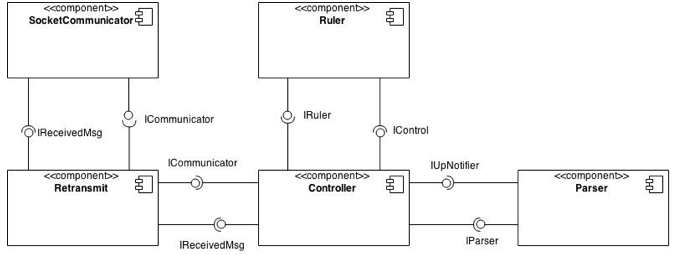
\includegraphics[scale=0.45]{include/diagrammeComposant1.png}
\end{frame}

\begin{frame}
  \frametitle{Architecture de la solution}
  \framesubtitle{Diagramme de composant 2 (final)}
  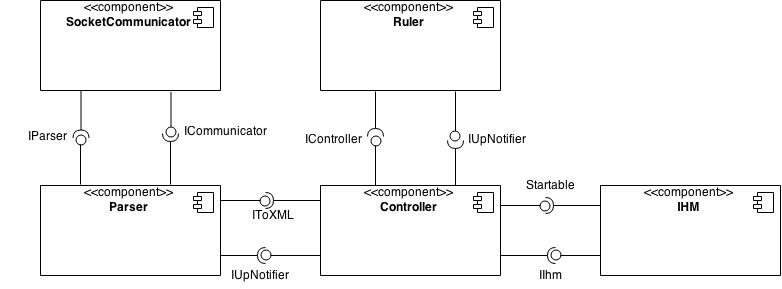
\includegraphics[scale=0.44]{include/diagrammeComposant2.jpg}
\end{frame}

%----------------------------------------------------

\begin{frame}
  \frametitle{Système de communication contrôleur/moniteur}
  \framesubtitle{Les phases des échanges contrôleur/moniteur}
  \begin{columns}[t]
    \begin{column}{0.5\textwidth}
      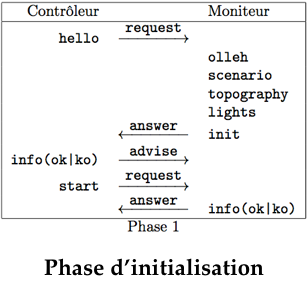
\includegraphics[scale=0.40]{include/phaseInit.png}
    \end{column}
    \begin{column}{0.5\textwidth}
      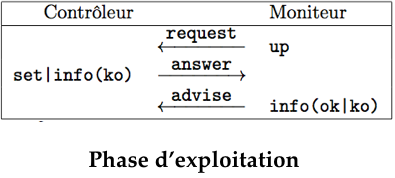
\includegraphics[scale=0.40]{include/phaseExpl.png}
    \end{column}
  \end{columns}
\end{frame}

%----------------------------------------------------

\begin{frame}
  \frametitle{Système de gestion des règles de circulation}
  \framesubtitle{1er Scénario}
  Circuit minimal
  \vspace{1em}
  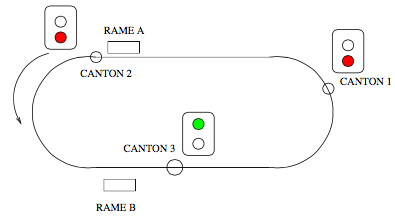
\includegraphics[scale=0.70]{include/scenario1.png}
\end{frame}

\begin{frame}
  \frametitle{Système de gestion des règles de circulation}
  \framesubtitle{2ème Scénario}
  Ajout des aiguillages 2-1
  \vspace{1em}
  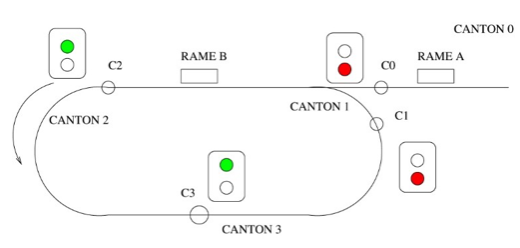
\includegraphics[scale=0.65]{include/scenario2.png}
\end{frame}

\begin{frame}
  \frametitle{Système de gestion des règles de circulation}
  \framesubtitle{3ème Scénario}
  Ajout des aiguillages 1-2 et des stations
  \vspace{1em}
  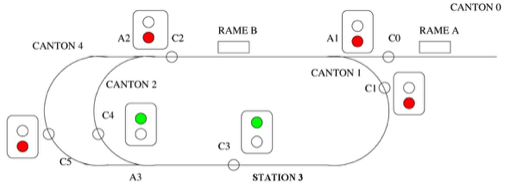
\includegraphics[scale=0.60]{include/scenario3.png}
\end{frame}

%----------------------------------------------------

\begin{frame}
  \frametitle{Interface graphique}
  \framesubtitle{Statique}
  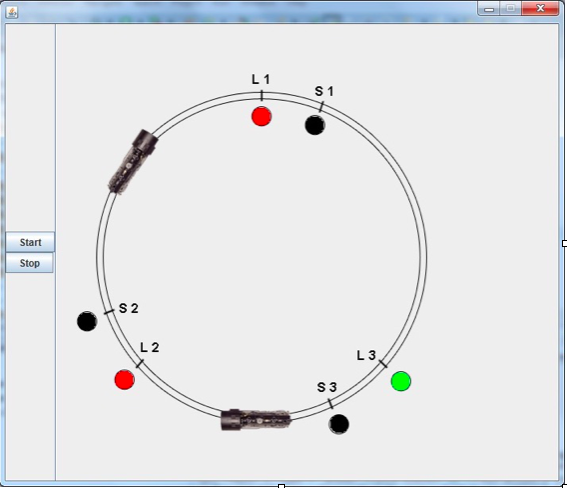
\includegraphics[scale=0.45]{include/ihmStat.png}
\end{frame}

%----------------------------------------------------

\begin{frame}
  \frametitle{Interface graphique}
  \framesubtitle{Dynamique}
  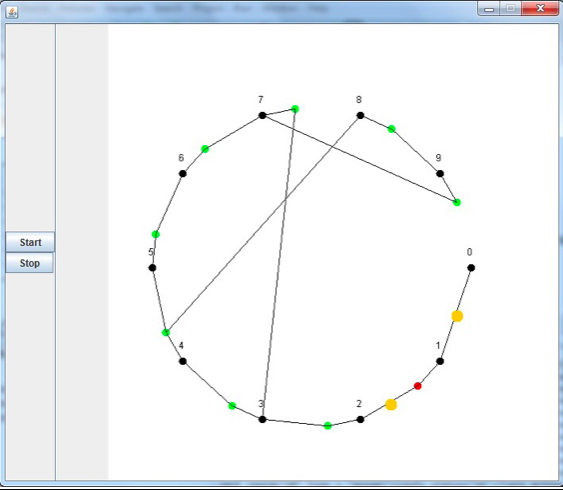
\includegraphics[scale=0.45]{include/ihmDyn.png}
\end{frame}
